\chapter{Background}


\section{Existing Applications}

% overview

There are a number of existing applications available that attempt to solve the problem posed by this project. These range from fitness applications to various navigation applications, which although may not be completely relevant to this project, do provide some similar features such as place recognition that will be useful to research.

Table \ref{table:existing-walking-apps} shows how well each of the existing applications related to this project have implemented certain features. The maximum score for the feature category is displayed in brackets. The full matrix detailing what aspects each feature category is split into and why the score was given to each app can be seen in Appendix \ref{appendix:existing-apps-matrices}.

\begin{table}[htb]
  \centering
  \begin{tabular}{|m{2cm}||c|c|c|c|c|c|}
    \hline
    Features & MapMyWalk & Strava & Let's Walk & Pok\'{e}mon Go & Citymapper & Google Maps\\
    \hline
    \hline
    Design (2) & 2 & 2 & 2 & 2 & 2 & 2\\
    \hline
    Ease of use (3) & 3 & 3 & 2 & 3 & 3 & 3\\
    \hline
    Tracking location (2) & 2 & 2 & 2 & 1 & 1 & 1\\
    \hline
    Navigation (4) & 3 & 1 & 1 & 2 & 1 & 3\\
    \hline
    Social interaction (5) & 2 & 2 & 2 & 0 & 0 & 0\\
    \hline
    \hline
    Total (16) & 12 & 10 & 9 & 8 & 7 & 9\\
    \hline
  \end{tabular}
  \caption{Matrix showing how well existing walking apps perform at given features}
  \label{table:existing-walking-apps}
\end{table}

The rest of this section discusses each application in detail, explaining their benefits and limitations. All of the applications are free to use unless stated otherwise.

% go through each existing app, discussing why they are good/bad with images

\subsection{MapMyWalk}

MapMyWalk \cite{Map} is a popular fitness application for iOS and Android that allows you to track your walks and compete against other users by completing challenges. 

The app also provides a premium subscription for \pounds4.49 per month, which gives you the ability to monitor your heart rate and set training goals designed to help you walk more.

\subsection{Strava}

\subsection{Let's Walk}

\subsection{Google Maps}

Although not a fitness application per say, Google Maps \cite{GoogleInc.} is one of the oldest services that provides route planning via different transport modes. The app contains current information about public transport, traffic and displays well-known cycling routes on map but there is little in the way of customisation for walking. When entering a destination, the app generates a route but users can also choose from a few different routes on map with the difference in time each one would take. However, no information is given as to whether a certain route is quieter than another, for example.

% add screenshot of walking route and time added on

\begin{figure}[hbt]
  \centering
  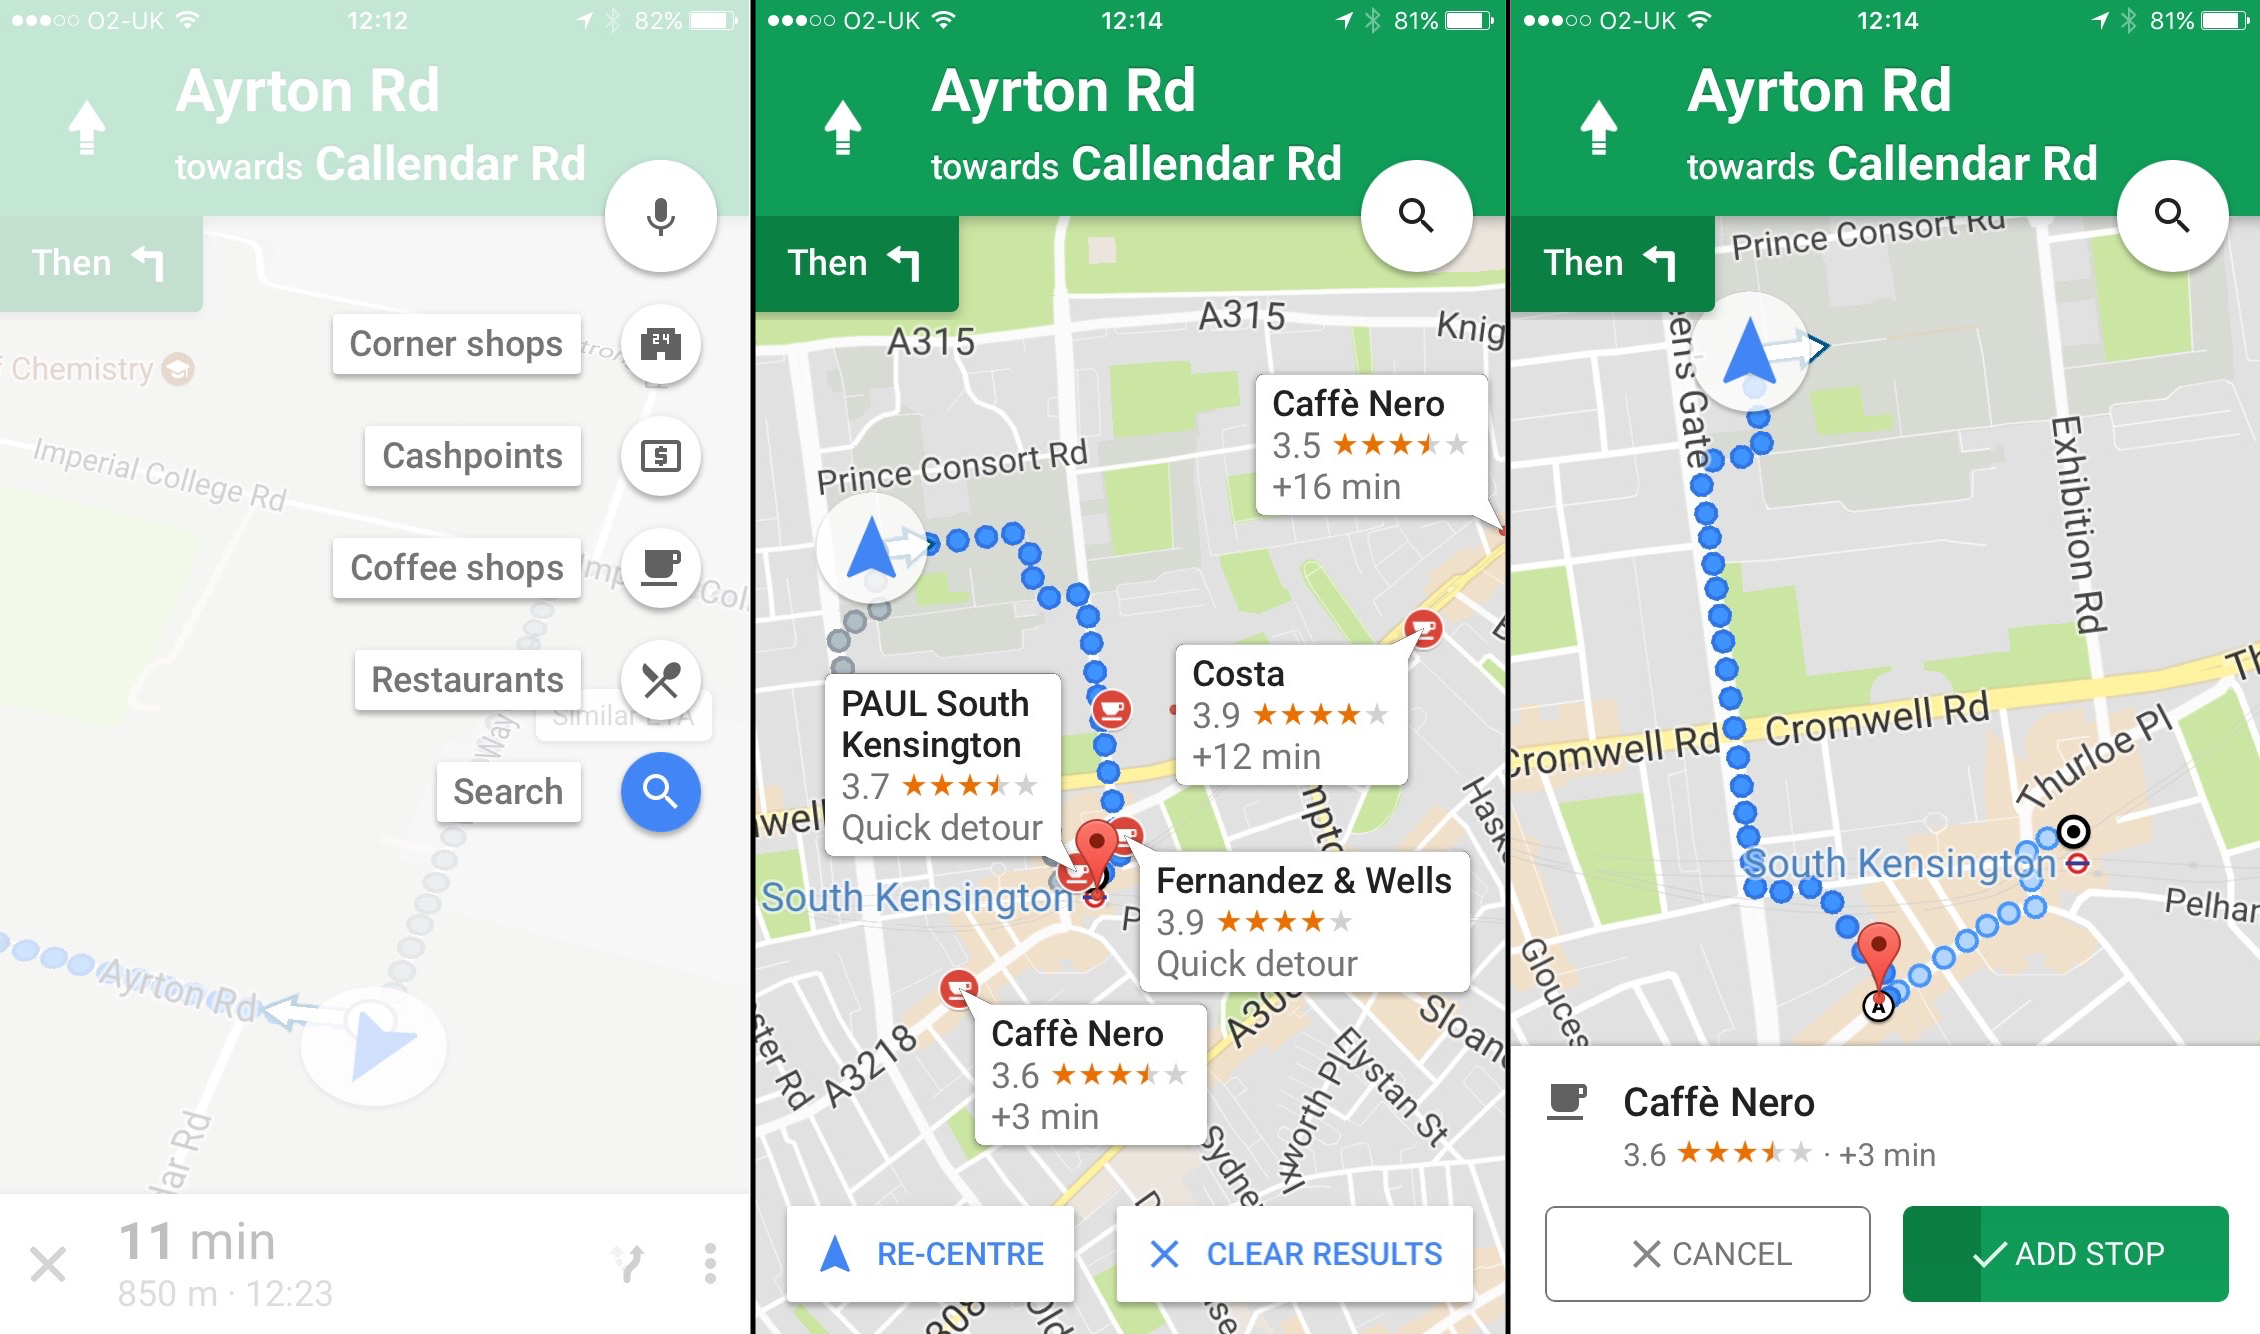
\includegraphics[width=0.9\textwidth]{google_maps_place_search}
  \caption{Adding places along your walking route in Google Maps for iOS. A list of categories to choose from (left) then shows all the places from within a search on a map (middle). A stop can then be added and the journey will be updated (right).}
  \label{google_maps_place_search}
\end{figure}


One feature of the Google Maps iOS application that is interesting to note is the places search along a route during a journey. Once a user has started a walking journey, they are able to search for places that are along the route. Google provides some categories of places to choose from, such as cashpoints and restaurants, but users can search for a specific place if they wish. The app will then display the results of the places search on the map showing how much additional time would be added on to your journey if you were to stop at a place, if any. One of more places can then be added to your journey and the walking directions will subsequently update to include these new stops. The full process of choosing a place category, selecting places on a map and stops being added to a journey can be seen in Figure \ref{google_maps_place_search}.

The places search feature is important as it is unique within any of the existing journey planner apps I have researched and it relates to one of my objectives regarding displaying points of interest when a user is on a walk (\textbf{Obj 3}). More research is conducted in Section *** to discover what tools these applications use to implement this feature.

\subsection{Citymapper}

Originating in London, Citymapper \cite{Citymapper} has become one of the leading journey planners for major cities around the world including Paris, Barcelona, New York, Tokyo and Sydney. 

\subsection{Pok\'{e}mon Go}

%\subsection{Walking Apps}

%There are a few existing applications that have

%\subsection{Navigation Apps}

% maybe don't include this
%Although existing navigation apps do not contain any features relating to tracking walks, they do provide information about how journeys and places are displayed on a map.


\section{Gamification}

% research how gamification has been used in applications, not just walking apps
% discuss how well each implementation has worked


% not sure whether to include this in background or design?
% think I will include general background on technologies here, and then which ones I chose in design
\section{Technologies}
%
\subsection{Operating System}
%
%\subsection{Web Server}
%
%\subsection{Database}
%

\subsection{Location Tracking}

% section on how to track calories burned?

\subsection{APIs}
